\subsection{Apparato sperimentale}\label{subsec:apparato-sperimentale}
  L’apparato sperimentale, riportato in [fig.1] è formato da un prisma
  posizionato al centro di una guida circolare graduata. Il prisma è montato
  ad un servomotore (??? modello) che gli permette di ruotare con una
  risoluzione angolare di 1.0° +/- 0.5°. (todo: il goniometro ha permesso di
  misurare l’angolo iniziale da cui far partire l’acquisizione). Un laser è
  puntato verso il cristallo, e due filtri polarizzatori sono posti in mezzo
  al fascio. Alla guida rotante è collegato un sensore di intensità luminosa
  (??? Modello).
  Il servo ed il sensore sono collegati a (?? mettere davvero tutto il setup
  oppure solamente una roba) una scheda arduino, che si occupa dell’acquisizione
  dei dati.
  (todo inserisci numeri della roba)

  Todo add specifiche di tutta la roba e link to datasheet.
  ADC arduino, reference voltage e cazzate varie
  Considerazioni su come l’errore sul sensore sia determinato principalmente da difficoltà nell’allineamento e da fluttuazioni del laser.

  \begin{figure}[h]
    \centering
    \caption{Apparato sperimentale e schema circuitale.}
    \begin{subfigure}{.4\textwidth}
      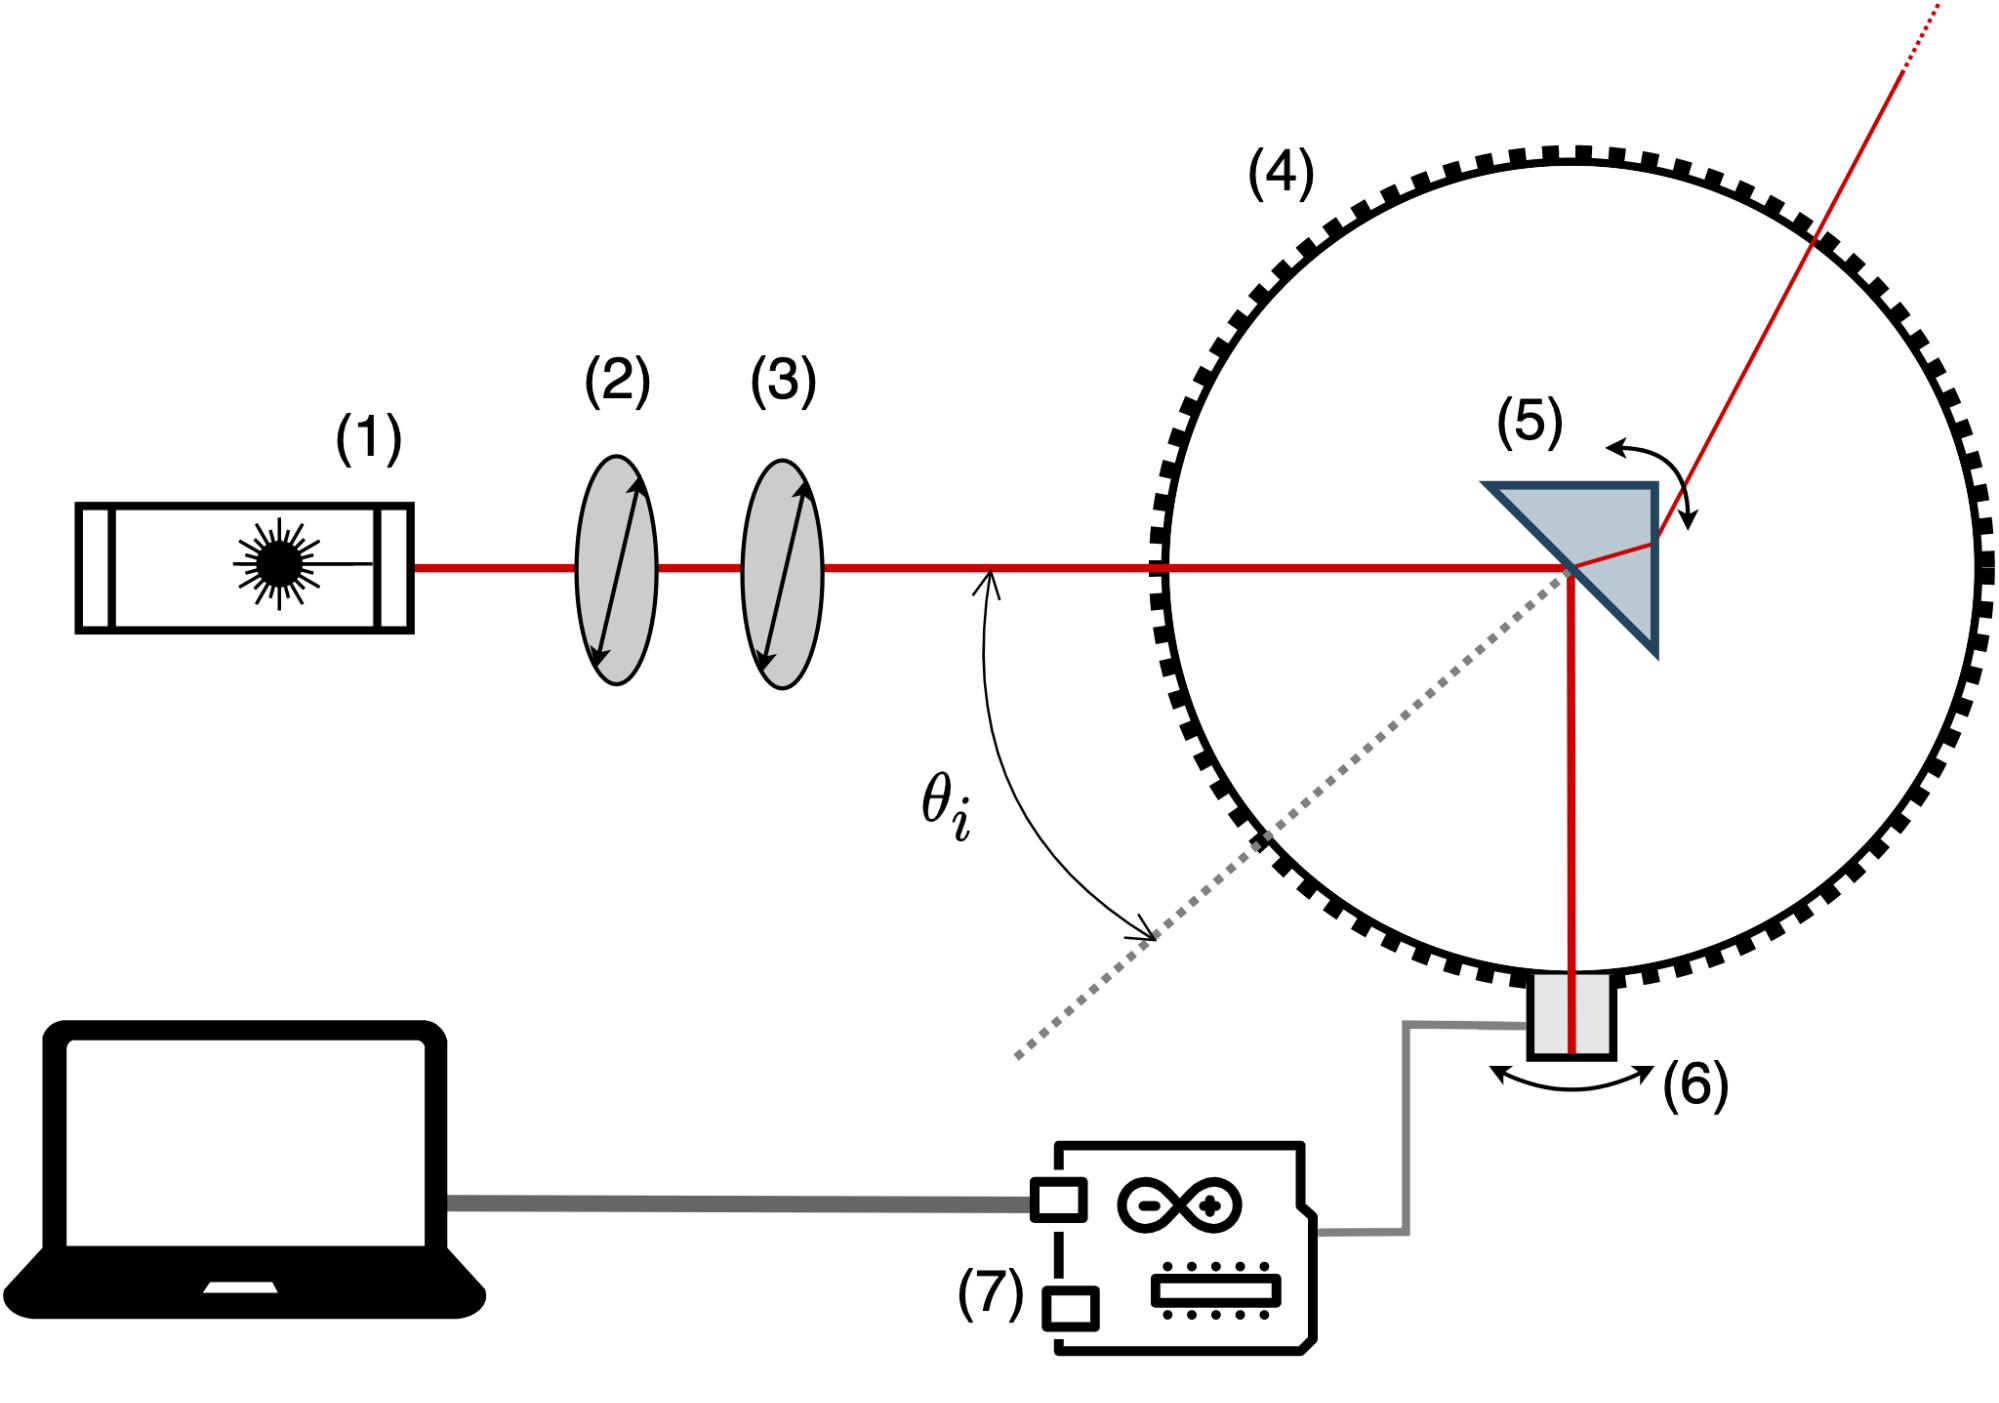
\includegraphics[width=7cm]{instrumental-apparatus.png}
      \caption{
        \emph{
          Apparato sperimentale. A partire da sinistra, in senso orario,
          si trovano: laser(1), filtri polaroid(2, 3), guida circolare(4),
          prisma(5), sensore(6), Arduino(7). Il servomotore non è riportato.
        }
      }
      \label{fig:instrumental-apparatus}
    \end{subfigure}%
    \hspace{20mm}
    \begin{subfigure}{.4\textwidth}
      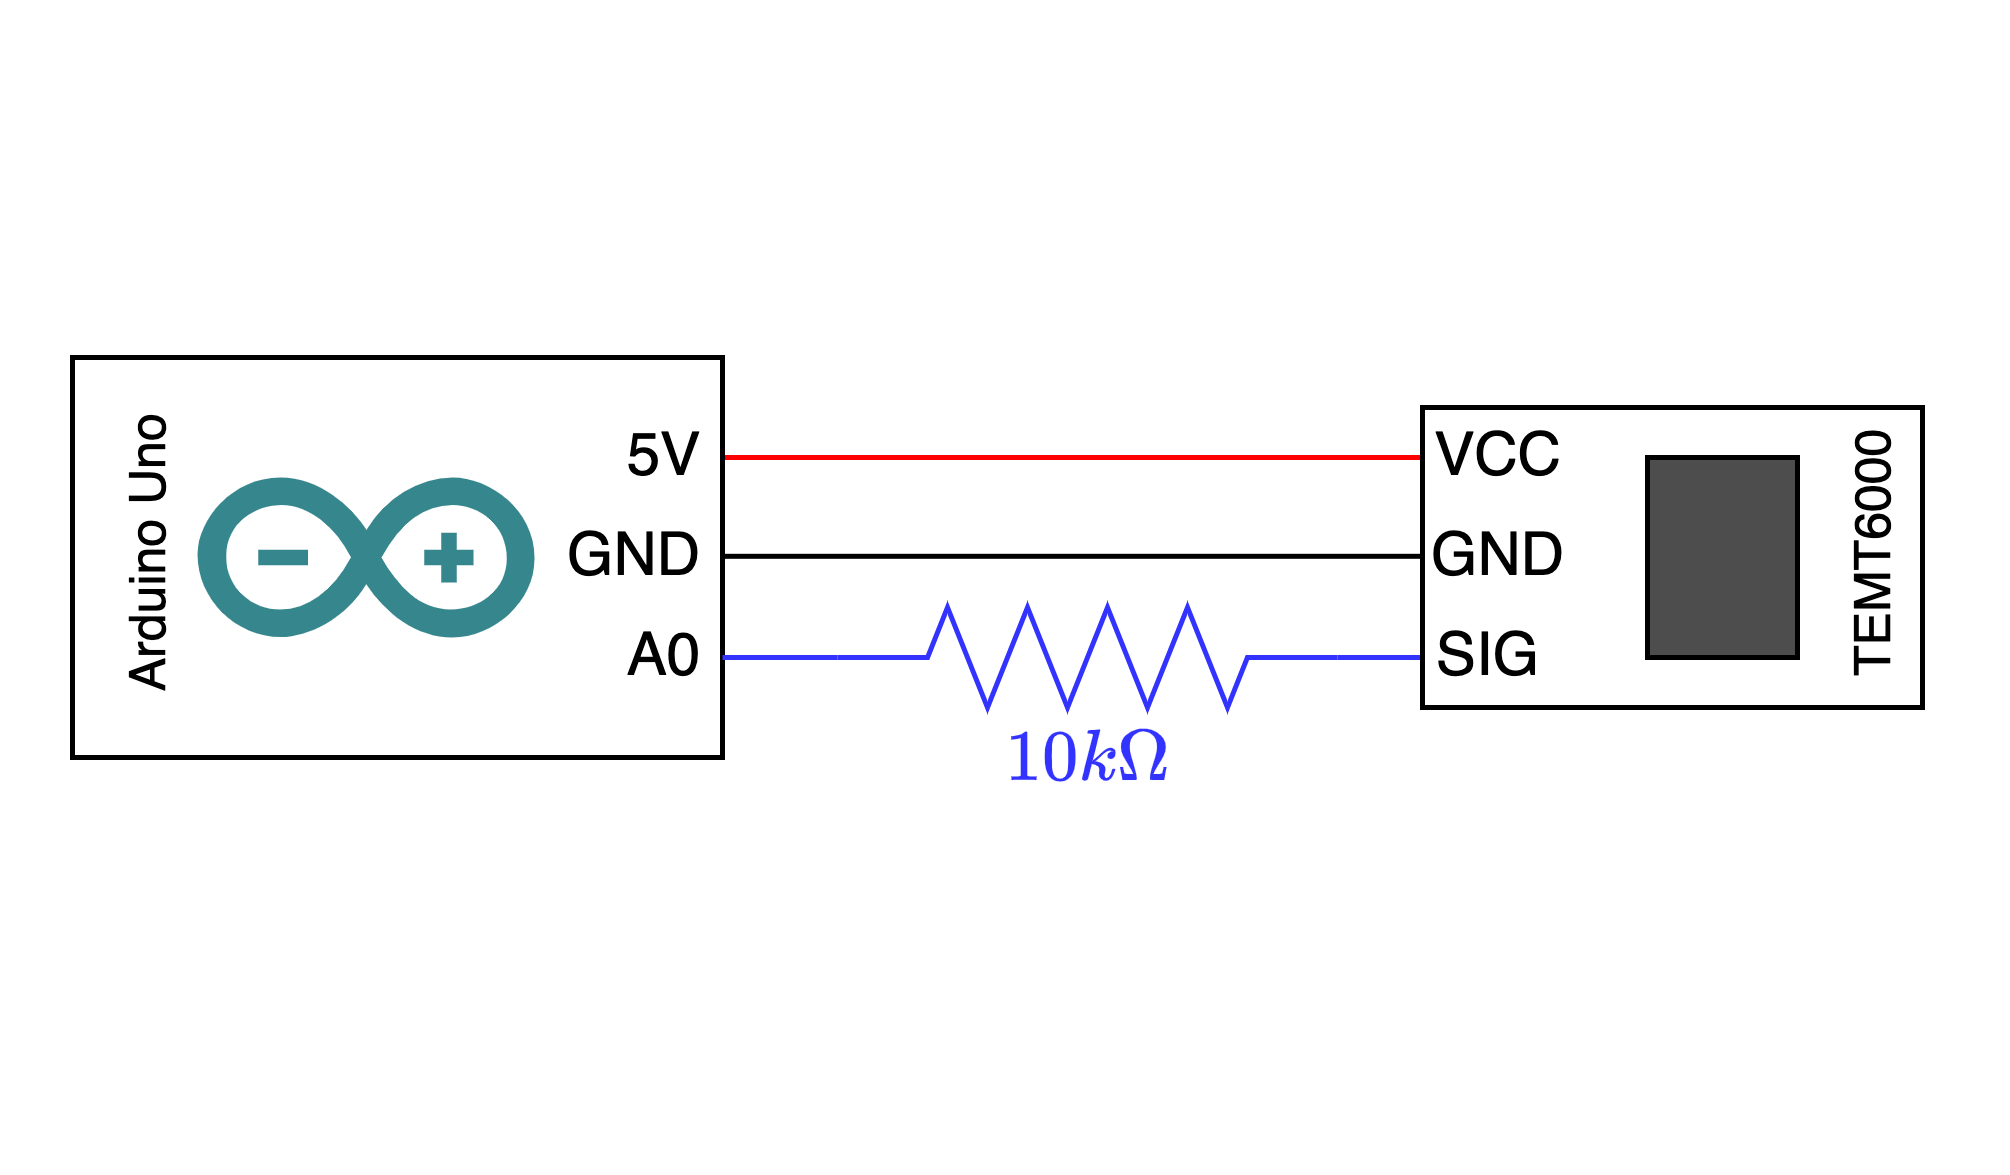
\includegraphics[width=7cm]{circuit-diagram.png}
      \caption{
        \emph{
          Schema circuitale. I pin $VCC$ e $GND$ del sensore sono collegati
          all'alimentazione di Arduino. Il pin $SIG$
          del sensore è collegato ad un input analogico di Arduino, tramite una
          resistenza da $10k\Omega$.
        }
      }
      \label{fig:circuit-diagram}
    \end{subfigure}
  \end{figure}

\subsection{Procedura sperimentale}\label{subsec:procedura-sperimentale}
  Abbiamo iniziato misurando l’andamento del coefficiente $R_\pi$. Partiamo posizionando il secondo polaroid in modo che la polarizzazione della luce sia parallela al lato del prisma. Il laser che abbiamo utilizzato emetteva luce polarizzata, quindi abbiamo dovuto aggiustare anche il suo angolo rispetto al polaroid. Prima di iniziare le misure, abbiamo regolato l’intensità del laser in modo che il sensore potesse rilevare un range di valori il più ampio possibile. Abbiamo quindi posizionato il sensore direttamente davanti al laser e abbiamo ruotato il primo filtro polaroid, fino a che il sensore non è riuscito a rilevare una variazione significativa di intensità.
  Per prendere le misure, abbiamo iniziato ruotando il prisma in modo da massimizzare $\theta_i$. Per raccogliere un
  punto dati abbiamo allineato il sensore con il fascio laser riflesso e ne abbiamo misurato l’intensità. Abbiamo
  ripetuto questa misura riducendo man mano il valore di $\theta_i$, fino ad arrivare il più vicino possibile a $0\deg$.
  Il nostro apparato sperimentale ci ha permesso di svolgere misure per ?? < $\theta_i$ < ??.
  Abbiamo poi ruotato il secondo polaroid di 90° e ripetuta la stessa procedura per misurare $R_\sigma$.
  In questo modo, abbiamo ottenuto le misure di intensità riflessa $I_\pi$ e $I_\sigma$ [fig ??]. Per ottenere i
  coefficienti di Fresnel, abbiamo normalizzato i dati ottenuti tenendo conto che:
  there is no difference between Rp and Rs at normal incidence
  at glancing angle in the less-dense medium the reflection coefficients are ±1,
  Come descritto in [Lipson]
  Da queste misure abbiamo ricavato anche l’angolo di Brewster, osservando per quale valore di $\theta_i$
  l’intensità $I_\pi$ si annulla.
\endinput
